\documentclass[11pt, oneside]{article}   	% use "amsart" instead of "article" for AMSLaTeX format
\usepackage{geometry}                		% See geometry.pdf to learn the layout options. There are lots.
\geometry{letterpaper}                   		% ... or a4paper or a5paper or ... 
%\geometry{landscape}                		% Activate for for rotated page geometry
%\usepackage[parfill]{parskip}    		% Activate to begin paragraphs with an empty line rather than an indent
\usepackage{graphicx}				% Use pdf, png, jpg, or eps with pdflatex; use eps in DVI mode
								% TeX will automatically convert eps --> pdf in pdflatex		
\usepackage{amssymb}
\usepackage{listings}
\graphicspath{{/Users/telliott_admin/Dropbox/Tex/png/}}

\title{Properties of the logarithm}
%\author{The Author}
\date{}							% Activate to display a given date or no date

\begin{document}
\maketitle
%\section{}
%\subsection{}
\large
This comes straight from David Jerrison's lecture in Calculus 1.  We define the logarithm function as
\[ L(x) = \int_1^x \frac{dt}{t} \]
\begin{center}
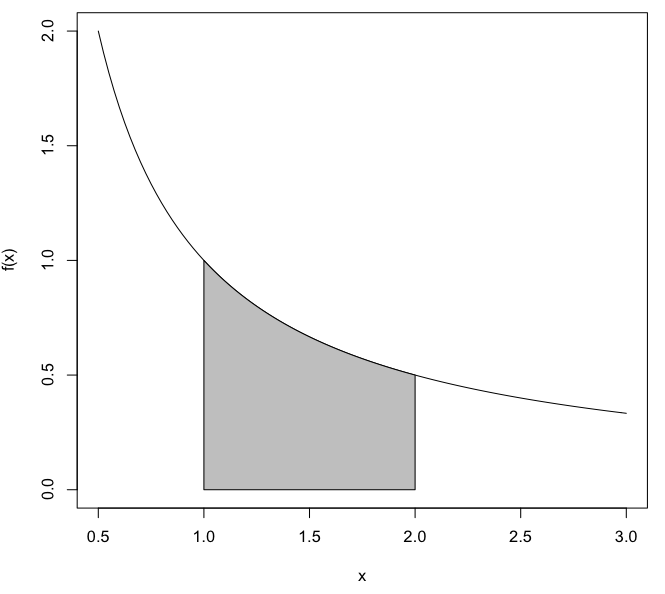
\includegraphics [scale=0.5] {inv.png}
\end{center}
The logarithm of $2$ is the area under the curve above, $f(x) = 1/x$, between $ 1 < x < 2$.
By the Fundamental Theorem of Calculus (part II) we have
\vspace{2 mm}

\noindent Property 1
\[ L'(x) = \frac{1}{x} \]
The slope of the logarithm function is always positive ($x>0$), but is undefined for $x=0$
\begin{center}
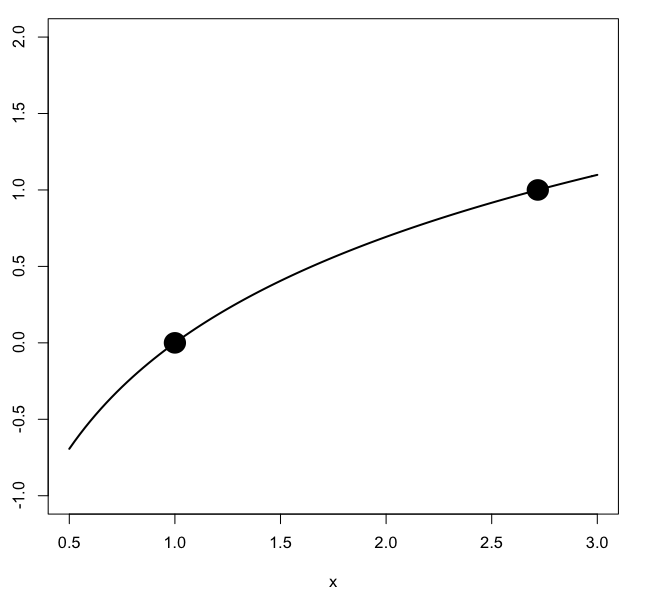
\includegraphics [scale=0.5] {log.png}
\end{center}
\vspace{2 mm}

\noindent Property 2
\[ L(1) = \int_1^1 \frac{dt}{t} = 0 \]
This property is by definition.  It fits with our use of exponents, where $b^0 = 1$.
\vspace{2 mm}

\noindent Property 3
\[ L''(x) = - \frac{1}{x^2} \]
Although the area under the curve $ln(x)$ is always increasing, so the slope is always positive, the rate of increase of the slope is always decreasing, so the shape is concave down.
\vspace{2 mm}

\noindent Property 4
\[ L(e) = 1 \]
This is by definition as well.  In extending to exponents it means we can write $y = ln(x) \iff e^y = x$.
\vspace{2 mm}

\noindent Property 5
\[ L(ab) = L(a) + L(b)  \]
To show that this last statement is true involves showing that this is equivalent
\[ \int_1^{ab} \frac{dt}{t} = \int_1^{a} \frac{dt}{t} + \int_a^{ab} \frac{dt}{t} \]
For the arguments $a$ and $ab$ we have 
\[ L(ab) = \int_1^{ab} \frac{dt}{t}   \]
\[ L(a) = \int_1^{a} \frac{dt}{t}   \]
Both of these are true by definition.  The one that takes a little work is
\[ L(b) = \int_a^{ab} \frac{dt}{t}   \]
Substitute $au=t$, then $a \ du = dt$ and
\[ L(b) = \int \frac{a \ du}{au} = \int \frac{du}{u}  \]
with a change in the limits
\[ t=a \Rightarrow u=1  \]
\[ t=ab \Rightarrow u=b  \]
So it's just
\[ L(b) = \int_1^b \frac{du}{u}  \]
which is again, true by definition.  So the function $L$ has the property that $L(ab) = L(a) + L(b)$, which is one of the two major properties of logarithms.

To see that the second is also true, start with
\[ L(a^r) = \int_1^{a^r} \frac{dt}{t}   \]
Substitute $t=u^r$, so $dt = ru^{r-1} du$, and the limits become 
\[ t=1 \Rightarrow u=1  \]
\[ t=a^r \Rightarrow u=a  \]
\[ L(a^r) = \int_{t=1}^{t=a^r} \frac{dt}{t} = \int_{u=1}^{u=a} \frac{1}{u^r} (ru^{r-1}) du = r \int_{u=1}^{u=a}  \frac{du}{u} = rL(a) \]
As Dunham says (using A for L) "these properties of the hyperbolic area---namely $A(ab) = A(a) + A(b)$ and $A(a^r) = rA(a)$---exactly mirror the corresponding properties of logarithms.  Clearly something interesting is afoot."

\subsection*{R code}

\begin{lstlisting}
f <- function(x) { return (1/x) }
plot(f, 0.5,3,cex=2,ylim=c(0,2))
xvals = seq(1,2,length=100)
yvals = f(xvals)
x = c(xvals,rev(xvals))
y = c(rep(0,100),rev(yvals))
polygon(x,y,col='gray')

f <- function(x) { return (log(x)) }
plot(f, 0.5,3,lwd=2,ylim=c(-1,2))
points(1,f(1),pch=16,cex=3)
points(2.71828,f(2.71828),pch=16,cex=3)
\end{lstlisting}

\end{document}  